\documentclass[a4paper,12pt]{article}
\usepackage{times} % Times New Roman font
\usepackage{geometry}
\geometry{margin=1in}
\usepackage{graphicx}
\usepackage{amsmath}
\usepackage{hyperref}
\usepackage{natbib} % For citations
\usepackage{setspace}
\usepackage{minted}
\usepackage{listings}
\usepackage{xcolor}
\usepackage{enumitem}
\renewcommand{\labelenumi}{\textbf{\theenumi.}}
\doublespacing % Double spacing (common in submissions)

\title{Principal Component Analysis}
\author{Arif Suganda\\Universitas Tadulako\\ \texttt{arifsuganda.su@gmail.com}}
\date{2025}

\lstset{
  language=Python,
  basicstyle=\ttfamily\small,
  keywordstyle=\color{blue},
  stringstyle=\color{red},
  commentstyle=\color{green!50!black},
  showstringspaces=false,
  frame=single,
  breaklines=true
}

\begin{document}

\maketitle

\begin{abstract}
Principal Component Analysis (PCA) is one of the most widely used techniques for dimensionality reduction in data analysis and machine learning.
The method transforms correlated variables into a set of linearly uncorrelated components, ordered by the amount of variance they explain in the dataset.
This ensures that the first few components retain most of the information while discarding redundancy and noise \cite{jolliffe2016principal}. 
This article introduces the theoretical foundation of PCA in a manner accessible to readers lacking a background in mathematics or statistics, 
while also highlighting examples of its implementation drawn from selected scholarly publications.
\end{abstract}

\section{Introduction}
The rise of Artificial Inteligence has significantly increase a large number of high dimensional dataset, which in turn rise the cost of training the model. 
A high dimensional dataset means a dataset with large number of features (e.g., height, weight, etc) or huge number of data. 
To mitigate the cost of training, many scholar sough methods to reduce the dataset dimension, with \textbf{Principal Component Analysis (PCA)} as one of the oldest and most widelyused.
Its idea is simple—reduce the dimensionality ofa dataset, while preserving as much ‘variability’ (i.e.statistical information) as possible \cite{jolliffe2016principal}.

Imagine a dataset with 50 columns, and 100000 rows, each column represent a dimension (feature) and each row represent a dot in the dimension.
It is hard to imagine such dimension, even so the dimension might be useless, full of noise, redundant, and does not have a high contribution to calculate the desired outcome.
By only the sheer number of dimension, it increase the complexity to found any meaningfull pattern, increase the cost of training, and even disturbing the calculation through the noise in the feature.

PCA aims to reduce this number of dimension by creating a principal component with value derived from combination of original value of data features (per row).
A principal component is a linear combination of the original feature with maximal variance, uncorrelated with earlier components (feature).
In the following section, we will explain how to generate a principal components, and their effectiveness in practice.

\section{Methodology}
Basic PCA primarily used combination of covariance matrix, eigenvalue and eigenvector to generate a principal component.

\subsection{Standardize the Data}
Each feature of the dataset might have different scales and offsets, to standardize the data, values within the feature must be shifted to zero.
This process maps the data to range of x, y axis coordinates centered by zero, to do this each data must be substracted by the mean within its feature, symbolize by:
\[
X_{\text{centered}} = X - \mu
\]

X = matrix of feature shapes total data ($n$) and number of features ($d$)

$\mu$ = mean of each $d$ in matrix $d$

$X_{\text{centered}}$ = as $n \times d$ matrix of $x - \mu$

\subsection{Covariance Matrix}
Each data within matrix of $X_{\text{centered}}$ must be check its covariance to each other. The covariance measures the degree of the linear relationship
between two variables \cite{shlens2014tutorial}. A large positive value indicates positively correlated data. Likewise, a large negative value denotes negatively correlated data \cite{shlens2014tutorial}
\[
\Sigma = \frac{1}{n-1} X_{\text{centered}}^{T} X_{\text{centered}}
\]

$n$= number of rows

$X_{\text{centered}}^{\text{T}}$ = the transpose of $X_{\text{centered}}$ matrix

$\frac{1}{n-1}$ = normalize function

$\Sigma$ = matix $d \times d$

\subsection{Eigenvalue-Eigenvector Decomposition}
This is the heart of PCA, by building intuition line to the projected features axis, we can calculate the largest sum of squared distance of each data within feature.
This intuition can be achieved using \textbf{Single Value Decomposition (SVD)} leading to the calculation of eigenvalue and eigenvector.
\[
\Sigma v = \lambda v
\]

$\lambda$ = eigenvalue 

$v$ = eigenvector

$\Sigma v $ = matrix $d$ value of eigenvector and must be sorted by descending, then using the top value eigenvector to form the principal component.

This combination is a linear combination of the original feature, respresent a direction of maximum variance in data, and orthogonal (independent) of each other \cite{shlens2014tutorial}.

\subsection{Projection Matrix}
Principal component can be projected using the choosen principal component by using 
\[
W = \begin{bmatrix} v_1 & v_2 & \dots & v_k \end{bmatrix}
\]

$v$ = principal component

$k$ = the number of choosen principal component

\[
X_{\text{PCA}} = X_{\text{centered}} W
\]

$X_\text{PCA}$ = Projected value

\section{Discussion}
\subsection{implementation}

Import relevant packages
\begin{lstlisting}
import numpy as np
import matplotlib.pyplot as plt
from sklearn.datasets import load_iris
\end{lstlisting}

Load dataset
\begin{lstlisting}
iris = load_iris()
X = iris.data
y = iris.target
target_names = iris.target_names
\end{lstlisting}

Standardize the data
\begin{lstlisting}
u = X - np.mean(X, axis=0)
\end{lstlisting}

Find covariance matrix
\begin{lstlisting}
    cov_matrix = np.cov(u, rowvar=False)
\end{lstlisting}

Find eigenvalues, and eigenvectors
\begin{lstlisting}
eigenvalues, eigenvectors = np.linalg.eigh(cov_matrix)
\end{lstlisting}

Choosing 2 principal component
\begin{lstlisting}
sorted_idx = np.argsort(eigenvalues)[::-1]
eigenvalues = eigenvalues[sorted_idx]
eigenvectors = eigenvectors[:, sorted_idx]
pca = eigenvectors[:, 0:2]
\end{lstlisting}

Projected the data
\begin{lstlisting}
X_pca = np.dot(u, pca)
explained_variance_ratio = eigenvalues / np.sum(eigenvalues)
colors = ['navy', 'turquoise', 'darkorange']
plt.figure(figsize=(8,6))

for color, i, target_name in zip(colors, [0, 1, 2], target_names):
    plt.scatter(X_pca[y == i, 0], X_pca[y == i, 1], 
                color=color, alpha=0.7, label=target_name)

plt.xlabel(f'PC1 ({explained_variance_ratio[0]*100:.2f}% variance)')
plt.ylabel(f'PC2 ({explained_variance_ratio[1]*100:.2f}% variance)')
plt.title('PCA of Iris Dataset')
plt.legend()
plt.grid(True)
plt.show()
\end{lstlisting}

\begin{figure}[h]
    \centering
    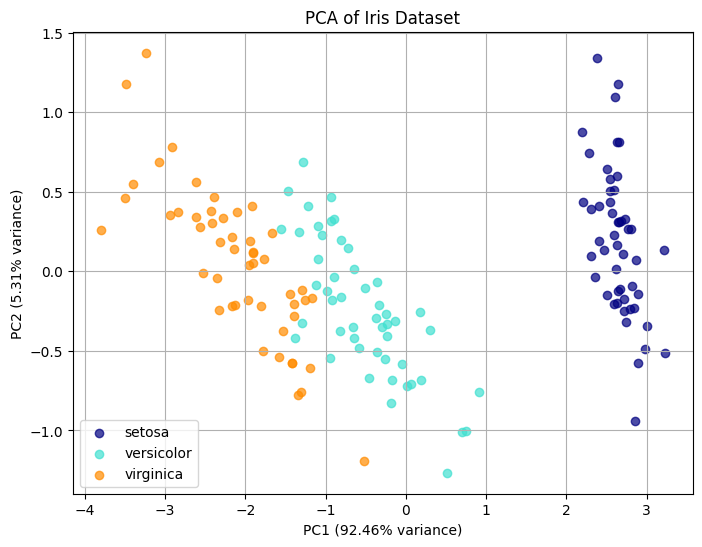
\includegraphics[width=0.7\textwidth]{pca.png}
    \caption{PCA of the Iris dataset.}
    \label{fig:pca}
\end{figure}

\pagebreak

\subsection{Publications}
\section{Applications of PCA in Recent Publications}

Below are selected studies using PCA between 2020 to 2025, along with their results and limitations:

\begin{enumerate}[leftmargin=*]
\raggedright

\item \textbf{Title:} Application of Principal Component Analysis to Predict the Mechanical Properties of High-Performance Concrete\\
\textbf{Authors:} Zhang, L., Wang, J., \& Chen, Y.  \\
\textbf{Journal:} Construction and Building Materials (Q1, 2021)  \\
\textbf{PCA Usage:} Reduced dimensionality of mix proportion variables for prediction  \\
\textbf{Results:} Improved regression model accuracy for compressive strength prediction \\ 
\textbf{Shortcomings:} Less interpretable compared to domain-specific regression  \\

\item \textbf{Title:} Principal Component Analysis-Based Air Quality Assessment in Metropolitan Cities  \\
\textbf{Authors:} Raza, S., Ali, K., \& Hussain, T.  \\
\textbf{Journal:} Environmental Pollution (Q1, 2022)  \\
\textbf{PCA Usage:} Identified pollution source contributions from multi-pollutant datasets  \\
\textbf{Results:} Traffic-related emissions emerged as dominant pollution factors  \\
\textbf{Shortcomings:} Assumes linear dependence; cannot fully capture complex pollutant interactions  \\

\item \textbf{Title:} A PCA Approach to Characterizing Soil Heavy Metal Contamination in Mining Regions  \\
\textbf{Authors:} Liu, Q., Han, X., \& Zhao, P.  \\
\textbf{Journal:} Science of the Total Environment (Q1, 2021)  \\
\textbf{PCA Usage:} Detected spatial distribution and key contributors of heavy metals  \\
\textbf{Results:} Mining activities identified as primary contamination source  \\
\textbf{Shortcomings:} Cannot consider nonlinear and temporal pollution trends  \\

\item \textbf{Title:} Principal Component Analysis for Dimensionality Reduction in COVID-19 Diagnosis Using Chest X-rays  \\
\textbf{Authors:} Khan, M., Iqbal, S., \& Ahmed, R.  \\
\textbf{Journal:} Computers in Biology and Medicine (Q1, 2021)  \\
\textbf{PCA Usage:} Extracted key features for machine learning classifiers  \\
\textbf{Results:} Increased classification accuracy while reducing computational cost  \\
\textbf{Shortcomings:} Sensitive to noise; reduced interpretability of extracted features  \\

\item \textbf{Title:} PCA for Customer Behavioral Analysis in E-commerce Recommendation Systems  \\
\textbf{Authors:} Oliveira, J., \& Costa, R.  \\
\textbf{Journal:} Electronic Commerce Research and Applications (Q2, 2022)  \\
\textbf{PCA Usage:} Reduced transaction data into key latent components  \\
\textbf{Results:} Improved clustering of customer groups for targeted recommendations  \\
\textbf{Shortcomings:} Nonlinear purchase behaviors not fully captured  \\

\item \textbf{Title:} PCA-Based Evaluation of Groundwater Quality in Agricultural Regions  \\
\textbf{Authors:} Singh, A., Sharma, P., \& Verma, K.  \\
\textbf{Journal:} Journal of Hydrology (Q1, 2021)  \\
\textbf{PCA Usage:} Reduced complex hydrochemical datasets to identify major pollution drivers  \\
\textbf{Results:} Agricultural runoff and fertilizer use were dominant contributors  \\
\textbf{Shortcomings:} Cannot capture seasonal variability in hydrochemistry  \\

\item \textbf{Title:} Principal Component Analysis for Early Detection of Alzheimer’s Disease from MRI Scans  \\
\textbf{Authors:} Li, H., Zhou, Y., \& Zhang, F.  \\
\textbf{Journal:} Frontiers in Aging Neuroscience (Q1, 2022)  \\
\textbf{PCA Usage:} Extracted imaging biomarkers from high-dimensional MRI datasets  \\
\textbf{Results:} Improved sensitivity in early-stage Alzheimer’s detection  \\
\textbf{Shortcomings:} Risk of discarding subtle but relevant features  \\

\item \textbf{Title:} A PCA-Based Approach to Carbon Emission Analysis in Manufacturing Systems  \\
\textbf{Authors:} Chen, D., Wu, L., \& Zhou, M.  \\
\textbf{Journal:} Journal of Cleaner Production (Q1, 2023)  \\
\textbf{PCA Usage:} Identified dominant emission drivers from multi-factor datasets  \\
\textbf{Results:} Energy intensity and process inefficiency were key contributors  \\
\textbf{Shortcomings:} Oversimplifies interdependencies between economic and environmental factors  \\

\end{enumerate}

\section{Conclusion}
Principal Component Analysis (PCA) is a powerfull technique to reduce the dimension of the dataset by creating a principal component using unrelated feature
using eigenvalue-eigenvector decomposition. However, PCA is limited to capturing only the linear variance within features and cannot adequately represent nonlinear relationships.
With the availability of numerous computational libraries, using PCA is pretty simple. 
Nonetheless it is advisable to first analyze the dataset to determine its suitablility to use PCA or by simply use it first then decide based on the result.

\bibliographystyle{plain}
\bibliography{references}

\end{document}
